% Created by tikzDevice version 0.6.2 on 2012-04-24 10:22:00
% !TEX encoding = UTF-8 Unicode
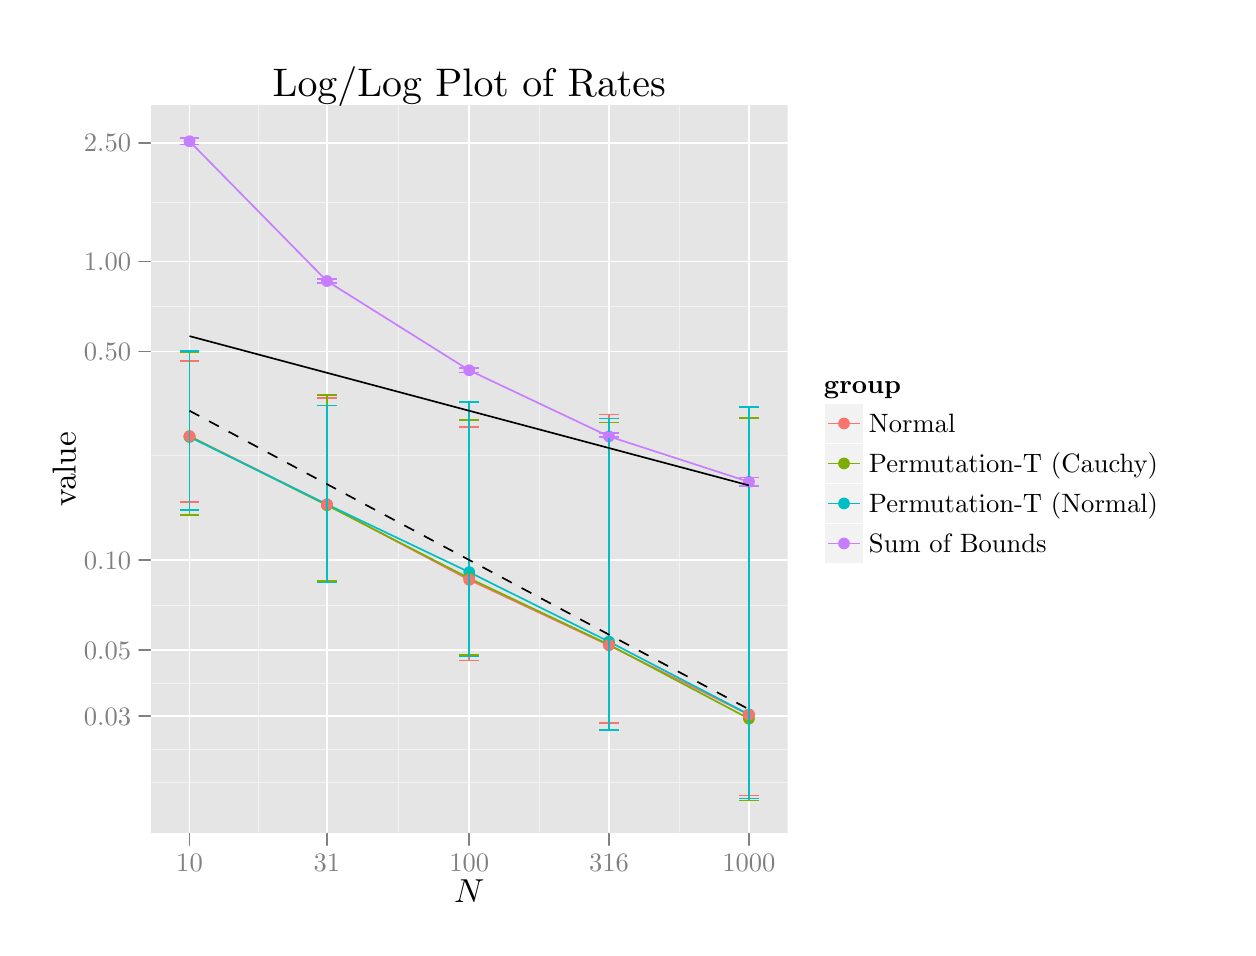
\begin{tikzpicture}[x=1pt,y=1pt]
\definecolor[named]{drawColor}{rgb}{0.00,0.00,0.00}
\definecolor[named]{fillColor}{rgb}{1.00,1.00,1.00}
\fill[color=fillColor,fill opacity=0.00,] (0,0) rectangle (433.62,325.21);
\begin{scope}
\path[clip] (  0.00,  0.00) rectangle (433.62,325.21);
\definecolor[named]{drawColor}{rgb}{0.41,0.16,0.58}
\end{scope}
\begin{scope}
\path[clip] (  0.00,  0.00) rectangle (433.62,325.21);
\definecolor[named]{drawColor}{rgb}{0.41,0.16,0.58}
\end{scope}
\begin{scope}
\path[clip] (  0.00,  0.00) rectangle (433.62,325.21);
\definecolor[named]{drawColor}{rgb}{0.41,0.16,0.58}
\end{scope}
\begin{scope}
\path[clip] (  0.00,  0.00) rectangle (433.62,325.21);
\definecolor[named]{drawColor}{rgb}{0.41,0.16,0.58}
\end{scope}
\begin{scope}
\path[clip] (  0.00,  0.00) rectangle (433.62,325.21);
\definecolor[named]{drawColor}{rgb}{0.41,0.16,0.58}
\end{scope}
\begin{scope}
\path[clip] (  0.00,  0.00) rectangle (433.62,325.21);
\definecolor[named]{drawColor}{rgb}{0.41,0.16,0.58}
\end{scope}
\begin{scope}
\path[clip] (  0.00,  0.00) rectangle (433.62,325.21);
\definecolor[named]{drawColor}{rgb}{0.41,0.16,0.58}
\end{scope}
\begin{scope}
\path[clip] (  0.00,  0.00) rectangle (433.62,325.21);
\definecolor[named]{drawColor}{rgb}{0.41,0.16,0.58}
\end{scope}
\begin{scope}
\path[clip] (  0.00,  0.00) rectangle (433.62,325.21);
\definecolor[named]{drawColor}{rgb}{0.41,0.16,0.58}
\end{scope}
\begin{scope}
\path[clip] (  0.00,  0.00) rectangle (433.62,325.21);
\definecolor[named]{drawColor}{rgb}{0.41,0.16,0.58}
\end{scope}
\begin{scope}
\path[clip] (  0.00,  0.00) rectangle (433.62,325.21);
\definecolor[named]{drawColor}{rgb}{0.41,0.16,0.58}
\end{scope}
\begin{scope}
\path[clip] (  0.00,  0.00) rectangle (433.62,325.21);
\definecolor[named]{drawColor}{rgb}{0.41,0.16,0.58}
\end{scope}
\begin{scope}
\path[clip] ( 44.49, 34.03) rectangle (274.61,297.23);
\definecolor[named]{drawColor}{rgb}{0.41,0.16,0.58}
\end{scope}
\begin{scope}
\path[clip] (  0.00,  0.00) rectangle (433.62,325.21);
\definecolor[named]{drawColor}{rgb}{0.41,0.16,0.58}
\end{scope}
\begin{scope}
\path[clip] (  0.00,  0.00) rectangle (433.62,325.21);
\definecolor[named]{drawColor}{rgb}{0.41,0.16,0.58}
\end{scope}
\begin{scope}
\path[clip] (  0.00,  0.00) rectangle (433.62,325.21);
\definecolor[named]{drawColor}{rgb}{0.41,0.16,0.58}
\end{scope}
\begin{scope}
\path[clip] (  0.00,  0.00) rectangle (433.62,325.21);
\definecolor[named]{drawColor}{rgb}{0.41,0.16,0.58}
\end{scope}
\begin{scope}
\path[clip] (  0.00,  0.00) rectangle (433.62,325.21);
\definecolor[named]{drawColor}{rgb}{0.41,0.16,0.58}
\end{scope}
\begin{scope}
\path[clip] (  0.00,  0.00) rectangle (433.62,325.21);
\definecolor[named]{drawColor}{rgb}{0.41,0.16,0.58}
\end{scope}
\begin{scope}
\path[clip] (  0.00,  0.00) rectangle (433.62,325.21);
\definecolor[named]{drawColor}{rgb}{0.41,0.16,0.58}
\end{scope}
\begin{scope}
\path[clip] (  0.00,  0.00) rectangle (433.62,325.21);
\definecolor[named]{drawColor}{rgb}{0.41,0.16,0.58}
\end{scope}
\begin{scope}
\path[clip] (  0.00,  0.00) rectangle (433.62,325.21);
\definecolor[named]{drawColor}{rgb}{0.41,0.16,0.58}
\end{scope}
\begin{scope}
\path[clip] (  0.00,  0.00) rectangle (433.62,325.21);
\definecolor[named]{drawColor}{rgb}{0.41,0.16,0.58}
\end{scope}
\begin{scope}
\path[clip] (  0.00,  0.00) rectangle (433.62,325.21);
\definecolor[named]{drawColor}{rgb}{0.41,0.16,0.58}
\end{scope}
\begin{scope}
\path[clip] (  0.00,  0.00) rectangle (433.62,325.21);
\definecolor[named]{drawColor}{rgb}{0.41,0.16,0.58}
\definecolor[named]{fillColor}{rgb}{1.00,1.00,1.00}

\draw[fill=fillColor,draw opacity=0.00,] (  0.00,  0.00) rectangle (433.62,325.21);
\end{scope}
\begin{scope}
\path[clip] (  0.00,  0.00) rectangle (433.62,325.21);
\definecolor[named]{drawColor}{rgb}{0.41,0.16,0.58}
\end{scope}
\begin{scope}
\path[clip] (  0.00,  0.00) rectangle (433.62,325.21);
\definecolor[named]{drawColor}{rgb}{0.41,0.16,0.58}
\definecolor[named]{drawColor}{rgb}{0.50,0.50,0.50}

\node[color=drawColor,anchor=base east,inner sep=0pt, outer sep=0pt, scale=  0.96] at ( 37.37, 73.13) {0.03};

\node[color=drawColor,anchor=base east,inner sep=0pt, outer sep=0pt, scale=  0.96] at ( 37.37, 97.07) {0.05};

\node[color=drawColor,anchor=base east,inner sep=0pt, outer sep=0pt, scale=  0.96] at ( 37.37,129.54) {0.10};

\node[color=drawColor,anchor=base east,inner sep=0pt, outer sep=0pt, scale=  0.96] at ( 37.37,204.94) {0.50};

\node[color=drawColor,anchor=base east,inner sep=0pt, outer sep=0pt, scale=  0.96] at ( 37.37,237.42) {1.00};

\node[color=drawColor,anchor=base east,inner sep=0pt, outer sep=0pt, scale=  0.96] at ( 37.37,280.34) {2.50};
\end{scope}
\begin{scope}
\path[clip] (  0.00,  0.00) rectangle (433.62,325.21);
\definecolor[named]{drawColor}{rgb}{0.41,0.16,0.58}
\definecolor[named]{drawColor}{rgb}{0.50,0.50,0.50}

\draw[color=drawColor,line width= 0.6pt,line cap=round,line join=round,fill opacity=0.00,] ( 40.22, 76.44) -- ( 44.49, 76.44);

\draw[color=drawColor,line width= 0.6pt,line cap=round,line join=round,fill opacity=0.00,] ( 40.22,100.37) -- ( 44.49,100.37);

\draw[color=drawColor,line width= 0.6pt,line cap=round,line join=round,fill opacity=0.00,] ( 40.22,132.85) -- ( 44.49,132.85);

\draw[color=drawColor,line width= 0.6pt,line cap=round,line join=round,fill opacity=0.00,] ( 40.22,208.25) -- ( 44.49,208.25);

\draw[color=drawColor,line width= 0.6pt,line cap=round,line join=round,fill opacity=0.00,] ( 40.22,240.72) -- ( 44.49,240.72);

\draw[color=drawColor,line width= 0.6pt,line cap=round,line join=round,fill opacity=0.00,] ( 40.22,283.65) -- ( 44.49,283.65);
\end{scope}
\begin{scope}
\path[clip] (  0.00,  0.00) rectangle (433.62,325.21);
\definecolor[named]{drawColor}{rgb}{0.41,0.16,0.58}
\end{scope}
\begin{scope}
\path[clip] (  0.00,  0.00) rectangle (433.62,325.21);
\definecolor[named]{drawColor}{rgb}{0.41,0.16,0.58}
\end{scope}
\begin{scope}
\path[clip] (  0.00,  0.00) rectangle (433.62,325.21);
\definecolor[named]{drawColor}{rgb}{0.41,0.16,0.58}
\end{scope}
\begin{scope}
\path[clip] (  0.00,  0.00) rectangle (433.62,325.21);
\definecolor[named]{drawColor}{rgb}{0.41,0.16,0.58}
\end{scope}
\begin{scope}
\path[clip] (  0.00,  0.00) rectangle (433.62,325.21);
\definecolor[named]{drawColor}{rgb}{0.41,0.16,0.58}
\end{scope}
\begin{scope}
\path[clip] ( 44.49, 34.03) rectangle (274.61,297.23);
\definecolor[named]{drawColor}{rgb}{0.41,0.16,0.58}
\definecolor[named]{fillColor}{rgb}{0.90,0.90,0.90}

\draw[fill=fillColor,draw opacity=0.00,] ( 44.49, 34.03) rectangle (274.61,297.23);
\definecolor[named]{drawColor}{rgb}{0.95,0.95,0.95}

\draw[color=drawColor,line width= 0.3pt,line cap=round,line join=round,fill opacity=0.00,] ( 44.49, 52.51) --
	(274.61, 52.51);

\draw[color=drawColor,line width= 0.3pt,line cap=round,line join=round,fill opacity=0.00,] ( 44.49, 64.47) --
	(274.61, 64.47);

\draw[color=drawColor,line width= 0.3pt,line cap=round,line join=round,fill opacity=0.00,] ( 44.49, 88.41) --
	(274.61, 88.41);

\draw[color=drawColor,line width= 0.3pt,line cap=round,line join=round,fill opacity=0.00,] ( 44.49,116.61) --
	(274.61,116.61);

\draw[color=drawColor,line width= 0.3pt,line cap=round,line join=round,fill opacity=0.00,] ( 44.49,170.55) --
	(274.61,170.55);

\draw[color=drawColor,line width= 0.3pt,line cap=round,line join=round,fill opacity=0.00,] ( 44.49,224.49) --
	(274.61,224.49);

\draw[color=drawColor,line width= 0.3pt,line cap=round,line join=round,fill opacity=0.00,] ( 44.49,262.19) --
	(274.61,262.19);

\draw[color=drawColor,line width= 0.3pt,line cap=round,line join=round,fill opacity=0.00,] ( 83.31, 34.03) --
	( 83.31,297.23);

\draw[color=drawColor,line width= 0.3pt,line cap=round,line join=round,fill opacity=0.00,] (133.85, 34.03) --
	(133.85,297.23);

\draw[color=drawColor,line width= 0.3pt,line cap=round,line join=round,fill opacity=0.00,] (184.80, 34.03) --
	(184.80,297.23);

\draw[color=drawColor,line width= 0.3pt,line cap=round,line join=round,fill opacity=0.00,] (235.33, 34.03) --
	(235.33,297.23);
\definecolor[named]{drawColor}{rgb}{1.00,1.00,1.00}

\draw[color=drawColor,line width= 0.6pt,line cap=round,line join=round,fill opacity=0.00,] ( 44.49, 76.44) --
	(274.61, 76.44);

\draw[color=drawColor,line width= 0.6pt,line cap=round,line join=round,fill opacity=0.00,] ( 44.49,100.37) --
	(274.61,100.37);

\draw[color=drawColor,line width= 0.6pt,line cap=round,line join=round,fill opacity=0.00,] ( 44.49,132.85) --
	(274.61,132.85);

\draw[color=drawColor,line width= 0.6pt,line cap=round,line join=round,fill opacity=0.00,] ( 44.49,208.25) --
	(274.61,208.25);

\draw[color=drawColor,line width= 0.6pt,line cap=round,line join=round,fill opacity=0.00,] ( 44.49,240.72) --
	(274.61,240.72);

\draw[color=drawColor,line width= 0.6pt,line cap=round,line join=round,fill opacity=0.00,] ( 44.49,283.65) --
	(274.61,283.65);

\draw[color=drawColor,line width= 0.6pt,line cap=round,line join=round,fill opacity=0.00,] ( 58.48, 34.03) --
	( 58.48,297.23);

\draw[color=drawColor,line width= 0.6pt,line cap=round,line join=round,fill opacity=0.00,] (108.14, 34.03) --
	(108.14,297.23);

\draw[color=drawColor,line width= 0.6pt,line cap=round,line join=round,fill opacity=0.00,] (159.55, 34.03) --
	(159.55,297.23);

\draw[color=drawColor,line width= 0.6pt,line cap=round,line join=round,fill opacity=0.00,] (210.05, 34.03) --
	(210.05,297.23);

\draw[color=drawColor,line width= 0.6pt,line cap=round,line join=round,fill opacity=0.00,] (260.62, 34.03) --
	(260.62,297.23);
\definecolor[named]{drawColor}{rgb}{0.97,0.46,0.43}

\draw[color=drawColor,line width= 0.6pt,line join=round,fill opacity=0.00,] ( 58.48,177.61) --
	(108.14,152.89) --
	(159.55,125.69) --
	(210.05,102.01) --
	(260.62, 76.96);
\definecolor[named]{drawColor}{rgb}{0.49,0.68,0.00}

\draw[color=drawColor,line width= 0.6pt,line join=round,fill opacity=0.00,] ( 58.48,177.55) --
	(108.14,152.64) --
	(159.55,126.25) --
	(210.05,102.26) --
	(260.62, 75.52);
\definecolor[named]{drawColor}{rgb}{0.00,0.75,0.77}

\draw[color=drawColor,line width= 0.6pt,line join=round,fill opacity=0.00,] ( 58.48,177.31) --
	(108.14,152.96) --
	(159.55,128.45) --
	(210.05,103.35) --
	(260.62, 77.05);
\definecolor[named]{drawColor}{rgb}{0.78,0.49,1.00}

\draw[color=drawColor,line width= 0.6pt,line join=round,fill opacity=0.00,] ( 58.48,284.15) --
	(108.14,233.65) --
	(159.55,201.40) --
	(210.05,177.51) --
	(260.62,161.10);
\definecolor[named]{fillColor}{rgb}{0.00,0.75,0.77}

\draw[fill=fillColor,draw opacity=0.00,] ( 58.48,177.31) circle (  2.13);
\definecolor[named]{fillColor}{rgb}{0.49,0.68,0.00}

\draw[fill=fillColor,draw opacity=0.00,] ( 58.48,177.55) circle (  2.13);
\definecolor[named]{fillColor}{rgb}{0.97,0.46,0.43}

\draw[fill=fillColor,draw opacity=0.00,] ( 58.48,177.61) circle (  2.13);
\definecolor[named]{fillColor}{rgb}{0.00,0.75,0.77}

\draw[fill=fillColor,draw opacity=0.00,] (108.14,152.96) circle (  2.13);
\definecolor[named]{fillColor}{rgb}{0.49,0.68,0.00}

\draw[fill=fillColor,draw opacity=0.00,] (108.14,152.64) circle (  2.13);
\definecolor[named]{fillColor}{rgb}{0.97,0.46,0.43}

\draw[fill=fillColor,draw opacity=0.00,] (108.14,152.89) circle (  2.13);
\definecolor[named]{fillColor}{rgb}{0.00,0.75,0.77}

\draw[fill=fillColor,draw opacity=0.00,] (159.55,128.45) circle (  2.13);
\definecolor[named]{fillColor}{rgb}{0.49,0.68,0.00}

\draw[fill=fillColor,draw opacity=0.00,] (159.55,126.25) circle (  2.13);
\definecolor[named]{fillColor}{rgb}{0.97,0.46,0.43}

\draw[fill=fillColor,draw opacity=0.00,] (159.55,125.69) circle (  2.13);
\definecolor[named]{fillColor}{rgb}{0.00,0.75,0.77}

\draw[fill=fillColor,draw opacity=0.00,] (210.05,103.35) circle (  2.13);
\definecolor[named]{fillColor}{rgb}{0.49,0.68,0.00}

\draw[fill=fillColor,draw opacity=0.00,] (210.05,102.26) circle (  2.13);
\definecolor[named]{fillColor}{rgb}{0.97,0.46,0.43}

\draw[fill=fillColor,draw opacity=0.00,] (210.05,102.01) circle (  2.13);
\definecolor[named]{fillColor}{rgb}{0.00,0.75,0.77}

\draw[fill=fillColor,draw opacity=0.00,] (260.62, 77.05) circle (  2.13);
\definecolor[named]{fillColor}{rgb}{0.49,0.68,0.00}

\draw[fill=fillColor,draw opacity=0.00,] (260.62, 75.52) circle (  2.13);
\definecolor[named]{fillColor}{rgb}{0.97,0.46,0.43}

\draw[fill=fillColor,draw opacity=0.00,] (260.62, 76.96) circle (  2.13);
\definecolor[named]{fillColor}{rgb}{0.78,0.49,1.00}

\draw[fill=fillColor,draw opacity=0.00,] ( 58.48,284.15) circle (  2.13);

\draw[fill=fillColor,draw opacity=0.00,] (108.14,233.65) circle (  2.13);

\draw[fill=fillColor,draw opacity=0.00,] (159.55,201.40) circle (  2.13);

\draw[fill=fillColor,draw opacity=0.00,] (210.05,177.51) circle (  2.13);

\draw[fill=fillColor,draw opacity=0.00,] (260.62,161.10) circle (  2.13);
\definecolor[named]{drawColor}{rgb}{0.97,0.46,0.43}

\draw[color=drawColor,line width= 0.6pt,line join=round,fill opacity=0.00,] ( 54.95,204.74) --
	( 62.02,204.74);

\draw[color=drawColor,line width= 0.6pt,line join=round,fill opacity=0.00,] ( 58.48,204.74) --
	( 58.48,153.80);

\draw[color=drawColor,line width= 0.6pt,line join=round,fill opacity=0.00,] ( 54.95,153.80) --
	( 62.02,153.80);

\draw[color=drawColor,line width= 0.6pt,line join=round,fill opacity=0.00,] (104.61,191.45) --
	(111.68,191.45);

\draw[color=drawColor,line width= 0.6pt,line join=round,fill opacity=0.00,] (108.14,191.45) --
	(108.14,125.00);

\draw[color=drawColor,line width= 0.6pt,line join=round,fill opacity=0.00,] (104.61,125.00) --
	(111.68,125.00);

\draw[color=drawColor,line width= 0.6pt,line join=round,fill opacity=0.00,] (156.01,181.01) --
	(163.09,181.01);

\draw[color=drawColor,line width= 0.6pt,line join=round,fill opacity=0.00,] (159.55,181.01) --
	(159.55, 96.56);

\draw[color=drawColor,line width= 0.6pt,line join=round,fill opacity=0.00,] (156.01, 96.56) --
	(163.09, 96.56);

\draw[color=drawColor,line width= 0.6pt,line join=round,fill opacity=0.00,] (206.51,185.42) --
	(213.59,185.42);

\draw[color=drawColor,line width= 0.6pt,line join=round,fill opacity=0.00,] (210.05,185.42) --
	(210.05, 73.96);

\draw[color=drawColor,line width= 0.6pt,line join=round,fill opacity=0.00,] (206.51, 73.96) --
	(213.59, 73.96);

\draw[color=drawColor,line width= 0.6pt,line join=round,fill opacity=0.00,] (257.08,184.36) --
	(264.15,184.36);

\draw[color=drawColor,line width= 0.6pt,line join=round,fill opacity=0.00,] (260.62,184.36) --
	(260.62, 47.72);

\draw[color=drawColor,line width= 0.6pt,line join=round,fill opacity=0.00,] (257.08, 47.72) --
	(264.15, 47.72);
\definecolor[named]{drawColor}{rgb}{0.49,0.68,0.00}

\draw[color=drawColor,line width= 0.6pt,line join=round,fill opacity=0.00,] ( 54.95,207.80) --
	( 62.02,207.80);

\draw[color=drawColor,line width= 0.6pt,line join=round,fill opacity=0.00,] ( 58.48,207.80) --
	( 58.48,149.16);

\draw[color=drawColor,line width= 0.6pt,line join=round,fill opacity=0.00,] ( 54.95,149.16) --
	( 62.02,149.16);

\draw[color=drawColor,line width= 0.6pt,line join=round,fill opacity=0.00,] (104.61,192.36) --
	(111.68,192.36);

\draw[color=drawColor,line width= 0.6pt,line join=round,fill opacity=0.00,] (108.14,192.36) --
	(108.14,125.24);

\draw[color=drawColor,line width= 0.6pt,line join=round,fill opacity=0.00,] (104.61,125.24) --
	(111.68,125.24);

\draw[color=drawColor,line width= 0.6pt,line join=round,fill opacity=0.00,] (156.01,183.42) --
	(163.09,183.42);

\draw[color=drawColor,line width= 0.6pt,line join=round,fill opacity=0.00,] (159.55,183.42) --
	(159.55, 98.53);

\draw[color=drawColor,line width= 0.6pt,line join=round,fill opacity=0.00,] (156.01, 98.53) --
	(163.09, 98.53);

\draw[color=drawColor,line width= 0.6pt,line join=round,fill opacity=0.00,] (206.51,182.54) --
	(213.59,182.54);

\draw[color=drawColor,line width= 0.6pt,line join=round,fill opacity=0.00,] (210.05,182.54) --
	(210.05, 71.65);

\draw[color=drawColor,line width= 0.6pt,line join=round,fill opacity=0.00,] (206.51, 71.65) --
	(213.59, 71.65);

\draw[color=drawColor,line width= 0.6pt,line join=round,fill opacity=0.00,] (257.08,184.20) --
	(264.15,184.20);

\draw[color=drawColor,line width= 0.6pt,line join=round,fill opacity=0.00,] (260.62,184.20) --
	(260.62, 46.00);

\draw[color=drawColor,line width= 0.6pt,line join=round,fill opacity=0.00,] (257.08, 46.00) --
	(264.15, 46.00);
\definecolor[named]{drawColor}{rgb}{0.00,0.75,0.77}

\draw[color=drawColor,line width= 0.6pt,line join=round,fill opacity=0.00,] ( 54.95,208.27) --
	( 62.02,208.27);

\draw[color=drawColor,line width= 0.6pt,line join=round,fill opacity=0.00,] ( 58.48,208.27) --
	( 58.48,150.80);

\draw[color=drawColor,line width= 0.6pt,line join=round,fill opacity=0.00,] ( 54.95,150.80) --
	( 62.02,150.80);

\draw[color=drawColor,line width= 0.6pt,line join=round,fill opacity=0.00,] (104.61,188.64) --
	(111.68,188.64);

\draw[color=drawColor,line width= 0.6pt,line join=round,fill opacity=0.00,] (108.14,188.64) --
	(108.14,124.72);

\draw[color=drawColor,line width= 0.6pt,line join=round,fill opacity=0.00,] (104.61,124.72) --
	(111.68,124.72);

\draw[color=drawColor,line width= 0.6pt,line join=round,fill opacity=0.00,] (156.01,189.99) --
	(163.09,189.99);

\draw[color=drawColor,line width= 0.6pt,line join=round,fill opacity=0.00,] (159.55,189.99) --
	(159.55, 98.00);

\draw[color=drawColor,line width= 0.6pt,line join=round,fill opacity=0.00,] (156.01, 98.00) --
	(163.09, 98.00);

\draw[color=drawColor,line width= 0.6pt,line join=round,fill opacity=0.00,] (206.51,183.95) --
	(213.59,183.95);

\draw[color=drawColor,line width= 0.6pt,line join=round,fill opacity=0.00,] (210.05,183.95) --
	(210.05, 71.48);

\draw[color=drawColor,line width= 0.6pt,line join=round,fill opacity=0.00,] (206.51, 71.48) --
	(213.59, 71.48);

\draw[color=drawColor,line width= 0.6pt,line join=round,fill opacity=0.00,] (257.08,188.23) --
	(264.15,188.23);

\draw[color=drawColor,line width= 0.6pt,line join=round,fill opacity=0.00,] (260.62,188.23) --
	(260.62, 46.65);

\draw[color=drawColor,line width= 0.6pt,line join=round,fill opacity=0.00,] (257.08, 46.65) --
	(264.15, 46.65);
\definecolor[named]{drawColor}{rgb}{0.78,0.49,1.00}

\draw[color=drawColor,line width= 0.6pt,line join=round,fill opacity=0.00,] ( 54.95,285.27) --
	( 62.02,285.27);

\draw[color=drawColor,line width= 0.6pt,line join=round,fill opacity=0.00,] ( 58.48,285.27) --
	( 58.48,283.02);

\draw[color=drawColor,line width= 0.6pt,line join=round,fill opacity=0.00,] ( 54.95,283.02) --
	( 62.02,283.02);

\draw[color=drawColor,line width= 0.6pt,line join=round,fill opacity=0.00,] (104.61,234.28) --
	(111.68,234.28);

\draw[color=drawColor,line width= 0.6pt,line join=round,fill opacity=0.00,] (108.14,234.28) --
	(108.14,233.01);

\draw[color=drawColor,line width= 0.6pt,line join=round,fill opacity=0.00,] (104.61,233.01) --
	(111.68,233.01);

\draw[color=drawColor,line width= 0.6pt,line join=round,fill opacity=0.00,] (156.01,202.24) --
	(163.09,202.24);

\draw[color=drawColor,line width= 0.6pt,line join=round,fill opacity=0.00,] (159.55,202.24) --
	(159.55,200.59);

\draw[color=drawColor,line width= 0.6pt,line join=round,fill opacity=0.00,] (156.01,200.59) --
	(163.09,200.59);

\draw[color=drawColor,line width= 0.6pt,line join=round,fill opacity=0.00,] (206.51,178.78) --
	(213.59,178.78);

\draw[color=drawColor,line width= 0.6pt,line join=round,fill opacity=0.00,] (210.05,178.78) --
	(210.05,177.26);

\draw[color=drawColor,line width= 0.6pt,line join=round,fill opacity=0.00,] (206.51,177.26) --
	(213.59,177.26);

\draw[color=drawColor,line width= 0.6pt,line join=round,fill opacity=0.00,] (257.08,162.61) --
	(264.15,162.61);

\draw[color=drawColor,line width= 0.6pt,line join=round,fill opacity=0.00,] (260.62,162.61) --
	(260.62,159.55);

\draw[color=drawColor,line width= 0.6pt,line join=round,fill opacity=0.00,] (257.08,159.55) --
	(264.15,159.55);
\definecolor[named]{drawColor}{rgb}{0.00,0.00,0.00}

\draw[color=drawColor,line width= 0.6pt,dash pattern=on 4pt off 4pt ,line join=round,fill opacity=0.00,] ( 58.48,186.78) --
	( 58.48,186.78) --
	( 58.48,186.78) --
	( 58.48,186.78) --
	(108.14,160.28) --
	(108.14,160.28) --
	(108.14,160.28) --
	(108.14,160.28) --
	(159.55,132.85) --
	(159.55,132.85) --
	(159.55,132.85) --
	(159.55,132.85) --
	(210.05,105.89) --
	(210.05,105.89) --
	(210.05,105.89) --
	(210.05,105.89) --
	(260.62, 78.91) --
	(260.62, 78.91) --
	(260.62, 78.91) --
	(260.62, 78.91);

\draw[color=drawColor,line width= 0.6pt,line join=round,fill opacity=0.00,] ( 58.48,213.75) --
	( 58.48,213.75) --
	( 58.48,213.75) --
	( 58.48,213.75) --
	(108.14,200.50) --
	(108.14,200.50) --
	(108.14,200.50) --
	(108.14,200.50) --
	(159.55,186.78) --
	(159.55,186.78) --
	(159.55,186.78) --
	(159.55,186.78) --
	(210.05,173.31) --
	(210.05,173.31) --
	(210.05,173.31) --
	(210.05,173.31) --
	(260.62,159.82) --
	(260.62,159.82) --
	(260.62,159.82) --
	(260.62,159.82);
\end{scope}
\begin{scope}
\path[clip] (  0.00,  0.00) rectangle (433.62,325.21);
\definecolor[named]{drawColor}{rgb}{0.41,0.16,0.58}
\end{scope}
\begin{scope}
\path[clip] (  0.00,  0.00) rectangle (433.62,325.21);
\definecolor[named]{drawColor}{rgb}{0.41,0.16,0.58}
\definecolor[named]{drawColor}{rgb}{0.50,0.50,0.50}

\node[color=drawColor,anchor=base,inner sep=0pt, outer sep=0pt, scale=  0.96] at ( 58.48, 20.31) {10};

\node[color=drawColor,anchor=base,inner sep=0pt, outer sep=0pt, scale=  0.96] at (108.14, 20.31) {31};

\node[color=drawColor,anchor=base,inner sep=0pt, outer sep=0pt, scale=  0.96] at (159.55, 20.31) {100};

\node[color=drawColor,anchor=base,inner sep=0pt, outer sep=0pt, scale=  0.96] at (210.05, 20.31) {316};

\node[color=drawColor,anchor=base,inner sep=0pt, outer sep=0pt, scale=  0.96] at (260.62, 20.31) {1000};
\end{scope}
\begin{scope}
\path[clip] (  0.00,  0.00) rectangle (433.62,325.21);
\definecolor[named]{drawColor}{rgb}{0.41,0.16,0.58}
\definecolor[named]{drawColor}{rgb}{0.50,0.50,0.50}

\draw[color=drawColor,line width= 0.6pt,line cap=round,line join=round,fill opacity=0.00,] ( 58.48, 29.77) -- ( 58.48, 34.03);

\draw[color=drawColor,line width= 0.6pt,line cap=round,line join=round,fill opacity=0.00,] (108.14, 29.77) -- (108.14, 34.03);

\draw[color=drawColor,line width= 0.6pt,line cap=round,line join=round,fill opacity=0.00,] (159.55, 29.77) -- (159.55, 34.03);

\draw[color=drawColor,line width= 0.6pt,line cap=round,line join=round,fill opacity=0.00,] (210.05, 29.77) -- (210.05, 34.03);

\draw[color=drawColor,line width= 0.6pt,line cap=round,line join=round,fill opacity=0.00,] (260.62, 29.77) -- (260.62, 34.03);
\end{scope}
\begin{scope}
\path[clip] (  0.00,  0.00) rectangle (433.62,325.21);
\definecolor[named]{drawColor}{rgb}{0.41,0.16,0.58}
\end{scope}
\begin{scope}
\path[clip] (  0.00,  0.00) rectangle (433.62,325.21);
\definecolor[named]{drawColor}{rgb}{0.41,0.16,0.58}
\end{scope}
\begin{scope}
\path[clip] (  0.00,  0.00) rectangle (433.62,325.21);
\definecolor[named]{drawColor}{rgb}{0.41,0.16,0.58}
\end{scope}
\begin{scope}
\path[clip] (  0.00,  0.00) rectangle (433.62,325.21);
\definecolor[named]{drawColor}{rgb}{0.41,0.16,0.58}
\definecolor[named]{drawColor}{rgb}{0.00,0.00,0.00}

\node[color=drawColor,anchor=base,inner sep=0pt, outer sep=0pt, scale=  1.44] at (159.55,300.24) {Log/Log Plot of Rates};
\end{scope}
\begin{scope}
\path[clip] (  0.00,  0.00) rectangle (433.62,325.21);
\definecolor[named]{drawColor}{rgb}{0.41,0.16,0.58}
\end{scope}
\begin{scope}
\path[clip] (  0.00,  0.00) rectangle (433.62,325.21);
\definecolor[named]{drawColor}{rgb}{0.41,0.16,0.58}
\definecolor[named]{drawColor}{rgb}{0.00,0.00,0.00}

\node[color=drawColor,anchor=base,inner sep=0pt, outer sep=0pt, scale=  1.20] at (159.55,  9.03) {$N$};
\end{scope}
\begin{scope}
\path[clip] (  0.00,  0.00) rectangle (433.62,325.21);
\definecolor[named]{drawColor}{rgb}{0.41,0.16,0.58}
\end{scope}
\begin{scope}
\path[clip] (  0.00,  0.00) rectangle (433.62,325.21);
\definecolor[named]{drawColor}{rgb}{0.41,0.16,0.58}
\definecolor[named]{drawColor}{rgb}{0.00,0.00,0.00}

\node[rotate= 90.00,color=drawColor,anchor=base,inner sep=0pt, outer sep=0pt, scale=  1.20] at ( 17.30,165.63) {value};
\end{scope}
\begin{scope}
\path[clip] (  0.00,  0.00) rectangle (433.62,325.21);
\definecolor[named]{drawColor}{rgb}{0.41,0.16,0.58}
\end{scope}
\begin{scope}
\path[clip] (  0.00,  0.00) rectangle (433.62,325.21);
\definecolor[named]{drawColor}{rgb}{0.41,0.16,0.58}
\end{scope}
\begin{scope}
\path[clip] (  0.00,  0.00) rectangle (433.62,325.21);
\definecolor[named]{drawColor}{rgb}{0.41,0.16,0.58}
\end{scope}
\begin{scope}
\path[clip] (  0.00,  0.00) rectangle (433.62,325.21);
\definecolor[named]{drawColor}{rgb}{0.41,0.16,0.58}
\end{scope}
\begin{scope}
\path[clip] (  0.00,  0.00) rectangle (433.62,325.21);
\definecolor[named]{drawColor}{rgb}{0.41,0.16,0.58}
\end{scope}
\begin{scope}
\path[clip] (  0.00,  0.00) rectangle (433.62,325.21);
\definecolor[named]{drawColor}{rgb}{0.41,0.16,0.58}
\end{scope}
\begin{scope}
\path[clip] (  0.00,  0.00) rectangle (433.62,325.21);
\definecolor[named]{drawColor}{rgb}{0.41,0.16,0.58}
\end{scope}
\begin{scope}
\path[clip] (  0.00,  0.00) rectangle (433.62,325.21);
\definecolor[named]{drawColor}{rgb}{0.41,0.16,0.58}
\end{scope}
\begin{scope}
\path[clip] (  0.00,  0.00) rectangle (433.62,325.21);
\definecolor[named]{drawColor}{rgb}{0.41,0.16,0.58}
\end{scope}
\begin{scope}
\path[clip] (  0.00,  0.00) rectangle (433.62,325.21);
\definecolor[named]{drawColor}{rgb}{0.41,0.16,0.58}
\end{scope}
\begin{scope}
\path[clip] (  0.00,  0.00) rectangle (433.62,325.21);
\definecolor[named]{drawColor}{rgb}{0.41,0.16,0.58}
\end{scope}
\begin{scope}
\path[clip] (  0.00,  0.00) rectangle (433.62,325.21);
\definecolor[named]{drawColor}{rgb}{0.41,0.16,0.58}
\end{scope}
\begin{scope}
\path[clip] (  0.00,  0.00) rectangle (433.62,325.21);
\definecolor[named]{drawColor}{rgb}{0.41,0.16,0.58}
\end{scope}
\begin{scope}
\path[clip] (  0.00,  0.00) rectangle (433.62,325.21);
\definecolor[named]{drawColor}{rgb}{0.41,0.16,0.58}
\end{scope}
\begin{scope}
\path[clip] (  0.00,  0.00) rectangle (433.62,325.21);
\definecolor[named]{drawColor}{rgb}{0.41,0.16,0.58}
\end{scope}
\begin{scope}
\path[clip] (  0.00,  0.00) rectangle (433.62,325.21);
\definecolor[named]{drawColor}{rgb}{0.41,0.16,0.58}
\end{scope}
\begin{scope}
\path[clip] (  0.00,  0.00) rectangle (433.62,325.21);
\definecolor[named]{drawColor}{rgb}{0.41,0.16,0.58}
\end{scope}
\begin{scope}
\path[clip] (  0.00,  0.00) rectangle (433.62,325.21);
\definecolor[named]{drawColor}{rgb}{0.41,0.16,0.58}
\end{scope}
\begin{scope}
\path[clip] (  0.00,  0.00) rectangle (433.62,325.21);
\definecolor[named]{drawColor}{rgb}{0.41,0.16,0.58}
\end{scope}
\begin{scope}
\path[clip] (  0.00,  0.00) rectangle (433.62,325.21);
\definecolor[named]{drawColor}{rgb}{0.41,0.16,0.58}
\end{scope}
\begin{scope}
\path[clip] (  0.00,  0.00) rectangle (433.62,325.21);
\definecolor[named]{drawColor}{rgb}{0.41,0.16,0.58}
\end{scope}
\begin{scope}
\path[clip] (  0.00,  0.00) rectangle (433.62,325.21);
\definecolor[named]{drawColor}{rgb}{0.41,0.16,0.58}
\end{scope}
\begin{scope}
\path[clip] (  0.00,  0.00) rectangle (433.62,325.21);
\definecolor[named]{drawColor}{rgb}{0.41,0.16,0.58}
\end{scope}
\begin{scope}
\path[clip] (  0.00,  0.00) rectangle (433.62,325.21);
\definecolor[named]{drawColor}{rgb}{0.41,0.16,0.58}
\end{scope}
\begin{scope}
\path[clip] (  0.00,  0.00) rectangle (433.62,325.21);
\definecolor[named]{drawColor}{rgb}{0.41,0.16,0.58}
\definecolor[named]{drawColor}{rgb}{1.00,1.00,1.00}

\draw[color=drawColor,line width= 0.6pt,line cap=round,line join=round,fill opacity=0.00,] (283.48,127.34) rectangle (412.71,203.93);
\end{scope}
\begin{scope}
\path[clip] (  0.00,  0.00) rectangle (433.62,325.21);
\definecolor[named]{drawColor}{rgb}{0.41,0.16,0.58}
\definecolor[named]{drawColor}{rgb}{0.00,0.00,0.00}

\node[color=drawColor,anchor=base west,inner sep=0pt, outer sep=0pt, scale=  0.96] at (287.75,193.03) {\bfseries group};
\end{scope}
\begin{scope}
\path[clip] (  0.00,  0.00) rectangle (433.62,325.21);
\definecolor[named]{drawColor}{rgb}{0.41,0.16,0.58}
\definecolor[named]{drawColor}{rgb}{1.00,1.00,1.00}
\definecolor[named]{fillColor}{rgb}{0.95,0.95,0.95}

\draw[color=drawColor,line width= 0.6pt,line cap=round,line join=round,fill=fillColor,] (287.75,174.97) rectangle (302.20,189.42);
\end{scope}
\begin{scope}
\path[clip] (  0.00,  0.00) rectangle (433.62,325.21);
\definecolor[named]{drawColor}{rgb}{0.41,0.16,0.58}
\definecolor[named]{drawColor}{rgb}{0.97,0.46,0.43}

\draw[color=drawColor,line width= 0.6pt,line join=round,fill opacity=0.00,] (289.20,182.19) -- (300.76,182.19);
\end{scope}
\begin{scope}
\path[clip] (  0.00,  0.00) rectangle (433.62,325.21);
\definecolor[named]{drawColor}{rgb}{0.41,0.16,0.58}
\definecolor[named]{fillColor}{rgb}{0.97,0.46,0.43}

\draw[fill=fillColor,draw opacity=0.00,] (294.98,182.19) circle (  2.13);
\end{scope}
\begin{scope}
\path[clip] (  0.00,  0.00) rectangle (433.62,325.21);
\definecolor[named]{drawColor}{rgb}{0.41,0.16,0.58}
\definecolor[named]{drawColor}{rgb}{0.97,0.46,0.43}

\draw[color=drawColor,line width= 0.6pt,line join=round,fill opacity=0.00,] (289.20,182.19) -- (300.76,182.19);
\end{scope}
\begin{scope}
\path[clip] (  0.00,  0.00) rectangle (433.62,325.21);
\definecolor[named]{drawColor}{rgb}{0.41,0.16,0.58}
\definecolor[named]{drawColor}{rgb}{1.00,1.00,1.00}
\definecolor[named]{fillColor}{rgb}{0.95,0.95,0.95}

\draw[color=drawColor,line width= 0.6pt,line cap=round,line join=round,fill=fillColor,] (287.75,160.51) rectangle (302.20,174.97);
\end{scope}
\begin{scope}
\path[clip] (  0.00,  0.00) rectangle (433.62,325.21);
\definecolor[named]{drawColor}{rgb}{0.41,0.16,0.58}
\definecolor[named]{drawColor}{rgb}{0.49,0.68,0.00}

\draw[color=drawColor,line width= 0.6pt,line join=round,fill opacity=0.00,] (289.20,167.74) -- (300.76,167.74);
\end{scope}
\begin{scope}
\path[clip] (  0.00,  0.00) rectangle (433.62,325.21);
\definecolor[named]{drawColor}{rgb}{0.41,0.16,0.58}
\definecolor[named]{fillColor}{rgb}{0.49,0.68,0.00}

\draw[fill=fillColor,draw opacity=0.00,] (294.98,167.74) circle (  2.13);
\end{scope}
\begin{scope}
\path[clip] (  0.00,  0.00) rectangle (433.62,325.21);
\definecolor[named]{drawColor}{rgb}{0.41,0.16,0.58}
\definecolor[named]{drawColor}{rgb}{0.49,0.68,0.00}

\draw[color=drawColor,line width= 0.6pt,line join=round,fill opacity=0.00,] (289.20,167.74) -- (300.76,167.74);
\end{scope}
\begin{scope}
\path[clip] (  0.00,  0.00) rectangle (433.62,325.21);
\definecolor[named]{drawColor}{rgb}{0.41,0.16,0.58}
\definecolor[named]{drawColor}{rgb}{1.00,1.00,1.00}
\definecolor[named]{fillColor}{rgb}{0.95,0.95,0.95}

\draw[color=drawColor,line width= 0.6pt,line cap=round,line join=round,fill=fillColor,] (287.75,146.06) rectangle (302.20,160.51);
\end{scope}
\begin{scope}
\path[clip] (  0.00,  0.00) rectangle (433.62,325.21);
\definecolor[named]{drawColor}{rgb}{0.41,0.16,0.58}
\definecolor[named]{drawColor}{rgb}{0.00,0.75,0.77}

\draw[color=drawColor,line width= 0.6pt,line join=round,fill opacity=0.00,] (289.20,153.29) -- (300.76,153.29);
\end{scope}
\begin{scope}
\path[clip] (  0.00,  0.00) rectangle (433.62,325.21);
\definecolor[named]{drawColor}{rgb}{0.41,0.16,0.58}
\definecolor[named]{fillColor}{rgb}{0.00,0.75,0.77}

\draw[fill=fillColor,draw opacity=0.00,] (294.98,153.29) circle (  2.13);
\end{scope}
\begin{scope}
\path[clip] (  0.00,  0.00) rectangle (433.62,325.21);
\definecolor[named]{drawColor}{rgb}{0.41,0.16,0.58}
\definecolor[named]{drawColor}{rgb}{0.00,0.75,0.77}

\draw[color=drawColor,line width= 0.6pt,line join=round,fill opacity=0.00,] (289.20,153.29) -- (300.76,153.29);
\end{scope}
\begin{scope}
\path[clip] (  0.00,  0.00) rectangle (433.62,325.21);
\definecolor[named]{drawColor}{rgb}{0.41,0.16,0.58}
\definecolor[named]{drawColor}{rgb}{1.00,1.00,1.00}
\definecolor[named]{fillColor}{rgb}{0.95,0.95,0.95}

\draw[color=drawColor,line width= 0.6pt,line cap=round,line join=round,fill=fillColor,] (287.75,131.60) rectangle (302.20,146.06);
\end{scope}
\begin{scope}
\path[clip] (  0.00,  0.00) rectangle (433.62,325.21);
\definecolor[named]{drawColor}{rgb}{0.41,0.16,0.58}
\definecolor[named]{drawColor}{rgb}{0.78,0.49,1.00}

\draw[color=drawColor,line width= 0.6pt,line join=round,fill opacity=0.00,] (289.20,138.83) -- (300.76,138.83);
\end{scope}
\begin{scope}
\path[clip] (  0.00,  0.00) rectangle (433.62,325.21);
\definecolor[named]{drawColor}{rgb}{0.41,0.16,0.58}
\definecolor[named]{fillColor}{rgb}{0.78,0.49,1.00}

\draw[fill=fillColor,draw opacity=0.00,] (294.98,138.83) circle (  2.13);
\end{scope}
\begin{scope}
\path[clip] (  0.00,  0.00) rectangle (433.62,325.21);
\definecolor[named]{drawColor}{rgb}{0.41,0.16,0.58}
\definecolor[named]{drawColor}{rgb}{0.78,0.49,1.00}

\draw[color=drawColor,line width= 0.6pt,line join=round,fill opacity=0.00,] (289.20,138.83) -- (300.76,138.83);
\end{scope}
\begin{scope}
\path[clip] (  0.00,  0.00) rectangle (433.62,325.21);
\definecolor[named]{drawColor}{rgb}{0.41,0.16,0.58}
\definecolor[named]{drawColor}{rgb}{0.00,0.00,0.00}

\node[color=drawColor,anchor=base west,inner sep=0pt, outer sep=0pt, scale=  0.96] at (304.01,178.89) {Normal};
\end{scope}
\begin{scope}
\path[clip] (  0.00,  0.00) rectangle (433.62,325.21);
\definecolor[named]{drawColor}{rgb}{0.41,0.16,0.58}
\definecolor[named]{drawColor}{rgb}{0.00,0.00,0.00}

\node[color=drawColor,anchor=base west,inner sep=0pt, outer sep=0pt, scale=  0.96] at (304.01,164.43) {Permutation-T (Cauchy)};
\end{scope}
\begin{scope}
\path[clip] (  0.00,  0.00) rectangle (433.62,325.21);
\definecolor[named]{drawColor}{rgb}{0.41,0.16,0.58}
\definecolor[named]{drawColor}{rgb}{0.00,0.00,0.00}

\node[color=drawColor,anchor=base west,inner sep=0pt, outer sep=0pt, scale=  0.96] at (304.01,149.98) {Permutation-T (Normal)};
\end{scope}
\begin{scope}
\path[clip] (  0.00,  0.00) rectangle (433.62,325.21);
\definecolor[named]{drawColor}{rgb}{0.41,0.16,0.58}
\definecolor[named]{drawColor}{rgb}{0.00,0.00,0.00}

\node[color=drawColor,anchor=base west,inner sep=0pt, outer sep=0pt, scale=  0.96] at (304.01,135.53) {Sum of Bounds};
\end{scope}
\begin{scope}
\path[clip] (  0.00,  0.00) rectangle (433.62,325.21);
\definecolor[named]{drawColor}{rgb}{0.41,0.16,0.58}
\end{scope}
\begin{scope}
\path[clip] (  0.00,  0.00) rectangle (433.62,325.21);
\definecolor[named]{drawColor}{rgb}{0.41,0.16,0.58}
\end{scope}
\begin{scope}
\path[clip] (  0.00,  0.00) rectangle (433.62,325.21);
\definecolor[named]{drawColor}{rgb}{0.41,0.16,0.58}
\end{scope}
\end{tikzpicture}
